\section{Projekt}
\subsection{Specyfikacja wymagań na produkt programowy}
Czy my tu musimy dać diagramy wymagań? :O
Diagram przypadków użycia

\begin{figure}[!htb]
  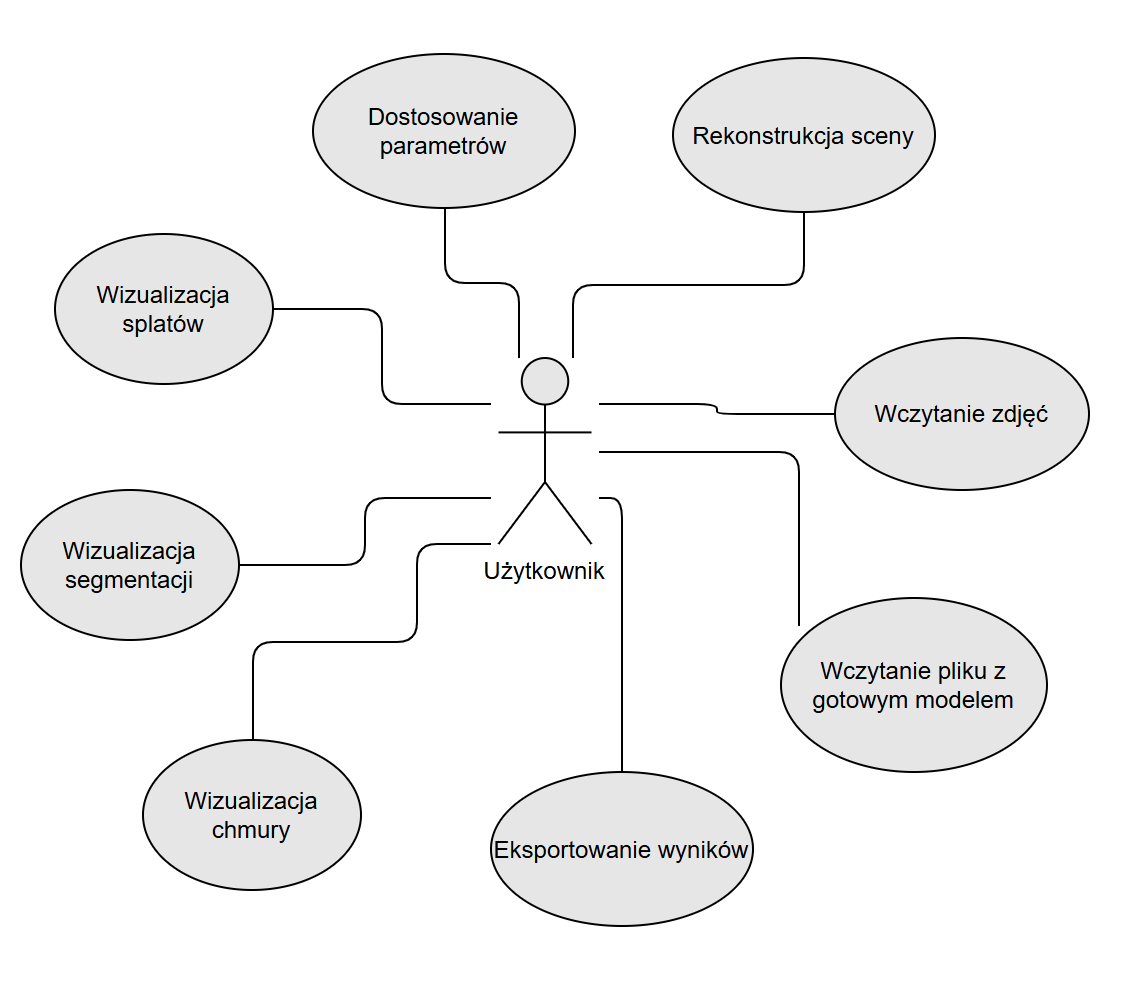
\includegraphics[width=\linewidth]{img/use_case_zpi.png}
  \caption{Diagram przypadków użycia}\label{fig:use_case_diagram}
\end{figure}

\subsection{Architektura}
Projekt architektury, zastosowane wzorce projektowe???
Jakiś język graficzny tutaj

\subsection{Implementacja}
Opis zastosowanych technologii i dokumentów

\subsubsection{Struktura plikowa projektu}

to wrzucić pod implementację

% millon opcji https://tex.stackexchange.com/questions/5073/making-a-simple-directory-tree
\begin{forest}
  for tree={
    grow'=0,
    child anchor=west,
    parent anchor=south,
    anchor=west,
    calign=first,
    edge path={
      \noexpand\path [draw, \forestoption{edge}] (!u.south west) ++(3pt,0) -- +(-3pt,0) |- (.child anchor)\forestoption{edge label};
    },
    before typesetting nodes={
      if n=1
        {insert before={[,phantom]}}
        {}
    },
    fit=band,
    before computing xy={l=15pt},
  }
[project
  [src
    [urb3d
      [rendering]
      [geometry]
      [models]
      [splats]
    ]
  ]
  [docs
    [main.pdf]
    [readme.txt]
  ]
  [config
    [config.json]
  ]
  [data
  [city\_model
        [images]
        [sparse
            [images.bin]
            [cameras.bin]
            [points.bin]
        ]
    ]
  ]
  [results
    [city\_model
      [experiment\_1
        [model.pt]
      ]
    ]
  ]
]
\end{forest}

\subsubsection{Gaussian Splatting}
W celu uruchomienia algorytmu Gaussian Splatting korzystamy z gotowej implementacji którą 
zapewnia biblioteka \href{https://docs.gsplat.studio/main/index.html}{\textit{gsplat}} \cite{ye2024gsplatopensourcelibrarygaussian}. Znajdują się w niej metody które odzwierciedlają wykonywane kroki w teoretycznym opisie algorytmu (np. \textit{rasterization}) a także dodatkowe elementy oparte na nowszych badaniach które usprawniają proces trenowania i renderowania (np. \textit{sparse gradient}, \textit{absgrad}, itp.). Dodatkowym plusem biblioteki jest wsparcie do renderowania dużych scen. Jej użycie wymaga posiadania karty graficznej CUDA.  

Jedną z naszych kontrybucji jest dostosowanie istniejącego skryptu trenującego \href{https://github.com/nerfstudio-project/gsplat/blob/main/examples/simple_trainer.py}{simple\_trainer} tak aby działał on poprawnie i zgodnie z naszymi wymaganiami. Przyjmuje on następujące argumenty:

% change style to not highlight python specific words
\lstset{style=basicstyle}
\begin{lstlisting}[language=SHELXL] 
  options:
  -h, --help            show this help message and exit
  --data_dir DATA_DIR   Path to the data directory.
  --result_dir RESULT_DIR
                        Path to the results directory.
  --data_factor DATA_FACTOR
                        Data factor.
  --init_type {sfm,random}
                        Initialization type.
  --strategy {default,mcmc}
                        Strategy type.
  --max_steps MAX_STEPS
                        Maximum number of steps.
  --init_num_pts INIT_NUM_PTS
                        Initial number of points (only for random).
  --delta_steps DELTA_STEPS
                        Delta steps for evaluation and saving.
  --scale_reg SCALE_REG
                        Scale regularization value.
  --opacity_reg OPACITY_REG
                        Opacity regularization value.
  --min_opacity MIN_OPACITY
                        Minimum opacity.
  --refine_stop_iter REFINE_STOP_ITER
                        Refinement stop iteration.
  --refine_every REFINE_EVERY
                        Refine frequency (iterations).
  --refine_start_iter REFINE_START_ITER
                        Refinement start iteration.
  --reset_every RESET_EVERY
                        Reset opacities every this steps. [strategy=default]
  --pause_refine_after_reset PAUSE_REFINE_AFTER_RESET
                        Pause refining GSs until this number of steps after reset. [strategy=default]
  --cap_max CAP_MAX     Maximum cap for MCMC gaussians. [strategy=mcmc]
  --sh_degree_interval SH_DEGREE_INTERVAL
                        Add spherical harmonics degree interval.
  --sh_degree {1,2,3}   Degree of spherical harmonics.
  --init_scale INIT_SCALE
                        Initial scale.
  --init_opa INIT_OPA   Initial opacity.
  --packed PACKED       Use packed mode for rasterization.
  --sparse_grad SPARSE_GRAD
                        Use sparse gradients for optimization.
\end{lstlisting}

\lstset{style=pythonstyle}

Z których obowiązkowe to \textit{data\_dir} - ścieżka do folderu z rekonstrukcją i zdjęciami i \textit{result\_dir} - ścieżka gdzie zostaną zapisane wyniki. 

\textbf{Opis parametrów}
\begin{itemize}
  \item \textit{data\_dir} - obowiązkowy; ścieżka do folderu z rekonstrukcją i zdjęciami
  \item \textit{result\_dir} - obowiązkowy; ścieżka gdzie zostaną zapisane wyniki
  \item init\_type - sposób inicjalizacji chmury punktów, losowy (random) lub z rekonstrukcji sfm (sfm)
  \item strategy - strategia zagęszczania gaussianów
  \item max\_steps - maksymalna liczba iteracji
  \item init\_num\_pts - początkowa liczba punktów dla sposobu inicjalizacji random
  \item delta\_steps - liczba iteracji po którch dokonywać ewaluacji oraz zapisu checkpointa
  \item scale\_reg - współczynnik regularyzacji skali gaussianów
  \item opacity\_reg - współczynnik regularyzacji przeźroczystości gaussianów
  \item min\_opacity - prog przeźroczystości poniżej którego splaty są odrzucane
  \item refine\_every - liczba iteracji po których następuje ulepszanie gaussianów wg. wybranej strategii 
  \item refine\_start\_iter - liczba iteracji od początku trenowania po której zachodzi pierwszy raz ulepszanie
  \item reset\_every - liczba iteracji po której zachodzi wyzerowanie przeźroczystości jeśli strategią jest \textit{default}
  \item pause\_refine\_after\_reset - liczba iteracji po wyzerowaniu które należy odczekać aby zaszedł krok doskonalenia gaussianów jeśli strategią jest \textit{default}
  \item cap\_max - maksymalna liczba gaussianów jeśli strategią jest \textit{mcmc}
  \item sh\_degree\_interval - liczba iteracji po której dodawany jest kolejny stopień zmiennych harmonicznych
  \item sh\_degree - stopień współczynników zmiennych harmonicznych 
  \item init\_scale - początkowa skala gaussianów 
  \item init\_opa - początkowa przeźroczystość gaussianów
\end{itemize}